\documentclass{slide}

\usepackage{pgfpages}
\setbeameroption{show notes on second screen}

\title{Architectural Decision Records}
\subtitle{Software Architecture}
\author{Richard Thomas}
\date{\week{2}}

\usepackage{languages}
\usepackage{changepage}

\hypersetup{
    colorlinks=true,
    linkcolor=violet,
    filecolor=purple,      
    urlcolor=blue,
    citecolor=black,
}

\begin{document}

\maketitle

\note[enumerate]{
    \item ADRs are the `why' of the architecture.
    \item Good if obvious approach is wrong.
    \item A mechanism for preserving the assumptions of an architecture.
}


\begin{frame}{Developer Reaction to Reading Software Architecture Documentation}

\begin{figure}
    \href{https://pixabay.com/vectors/computer-internet-unhappy-user-1295358/}{
\includegraphics[width=0.9\textwidth]{images/frustration.png}}
\end{figure}

\end{frame}

\note[enumerate]{
    \item ADRs follow on from views.
    \item But separated from views to make them more accessible.
}

\questionanswer{How do you know why certain decisions were made in the architectural design?}
{\highlight{Architectural Decision Records (ADRs)}}


\begin{frame}{Record Decisions that Influence}

\Large{
\begin{itemize}
    \item \highlight{Structure} of the architecture
    \item Delivery of \highlight{quality attributes}
    \item \highlight{Dependencies} between important parts of the architecture
	\vspace{1mm}
    \item \highlight{Interfaces} between important parts of the architecture
    \begin{itemize}
        \large{\item or external interfaces}
    \end{itemize}
    \item \highlight{Principles} about implementation techniques or platforms
\end{itemize}
}

\note{
    \begin{description}
        \item[Structure] e.g. \highlight{plugin} architecture because core platform expecting others to build or
        \highlight{microservices} architecture because of the need to scale and small teams.
        \item[Quality attributes] e.g. need to be \highlight{highly scalable} so we used cloud services.
        \item[Dependencies/Interfaces] we picked dependency Y, i.e. SMS API because rationale.
        ADRs don't record details of interface, just rationale.
        \item[Principles]
            \begin{itemize}
                \item use haskell because we get computer science grads.
                \item use on-prem because government org and have regulation.
                \item use language because of obsecure dependency.
            \end{itemize}
    \end{description}
}

\end{frame}

\begin{frame}

\begin{figure}
    \href{https://decodenatura.com/bad-comments-and-how-to-fix-them/}{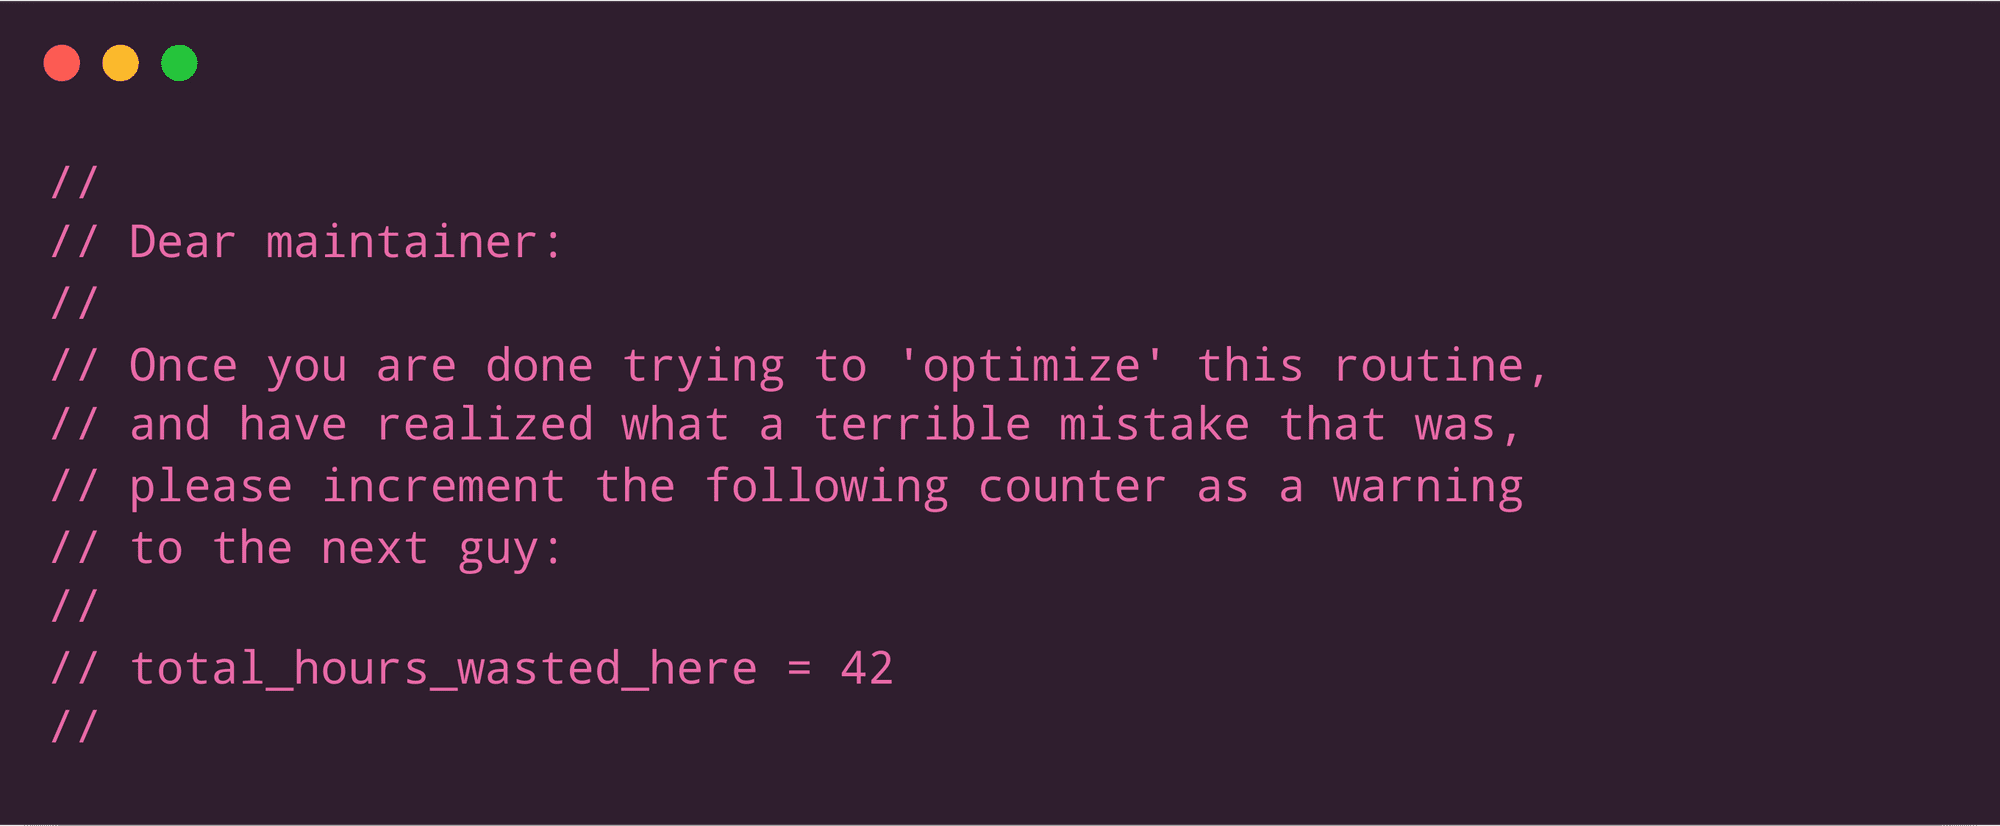
\includegraphics[width=0.9\textwidth]{images/warning-comment.png}}
\end{figure}

\end{frame}

\note{
    Can think of ADRs as warnings.

    Why is this not a good ADR? (no rationale)
}

\questionanswer{Why ADRs?}
{My code will defeat the architectural design,\\
\emph{if} I do not know why it was designed that way.}

\note{
    I will break things if I don't know why it works a certain way.

    I'll just \textsl{fix that}.
}

\point[ADRs]{Record a \highlight{single} decision}

\note[enumerate]{
\item Keeps it short.
\item More likely to write it (and read it).
}

\point[ADRs]{Are \highlight{never} deleted\\
Mark as \highlight{superseded} and link to new decision}

\note{
Preserves bad decisions --- less likely to repeat them.

Superseded decision: 1) that was a bad idea; 2) that was a good idea at the time but certain conditions have changed.
}

\questionanswer{Where are ADRs documented?}
{Each decision is a separate file in the project repository\footnote{See the \texttt{adrs} directory
in the \href{https://csse6400.uqcloud.net/resources/c4_model.zip}{C4 Model} on the course website.}}

\note{
C4 allows you to link to ADRs.

Useful to note as ADRs will be required for the project.
}


\begin{frame}{ADR Template \cite{nygard-adr}}

\Large{
\begin{description}
    \item[Title] Short phrase describing the decision
    \item[Date] When the decision was made
    \item[Status] Current status of the decision
    \begin{itemize}
        \large{\item proposed, accepted, deprecated, superseded, rejected}
    \end{itemize}
    \item[Summary] Summarise the decision and its rationale
    \item[Context] Describe the facts that influence the decision
    \item[Decision] Explain how the decision will solve the problem
    \item[Consequences] Impact of the decision
    \begin{itemize}
        \large{\item what's easier to do}
        \large{\item what's harder to do}
    \end{itemize}
\end{description}
}

\end{frame}

\note{
    \begin{description}
        \item[Title] Descriptive, easy to find, part of the filename.
        \item[Status] Rejected is an option --- prevents repeating proposals.
        \item[Summary] Describe context.
    \end{description}
}

\begin{frame}{ADR Example}

\begin{figure}
    \href{https://github.com/CSSE6400/software-architecture/blob/main/notes/views/c4_model/adrs/0001-independent-business-logic.md}
            {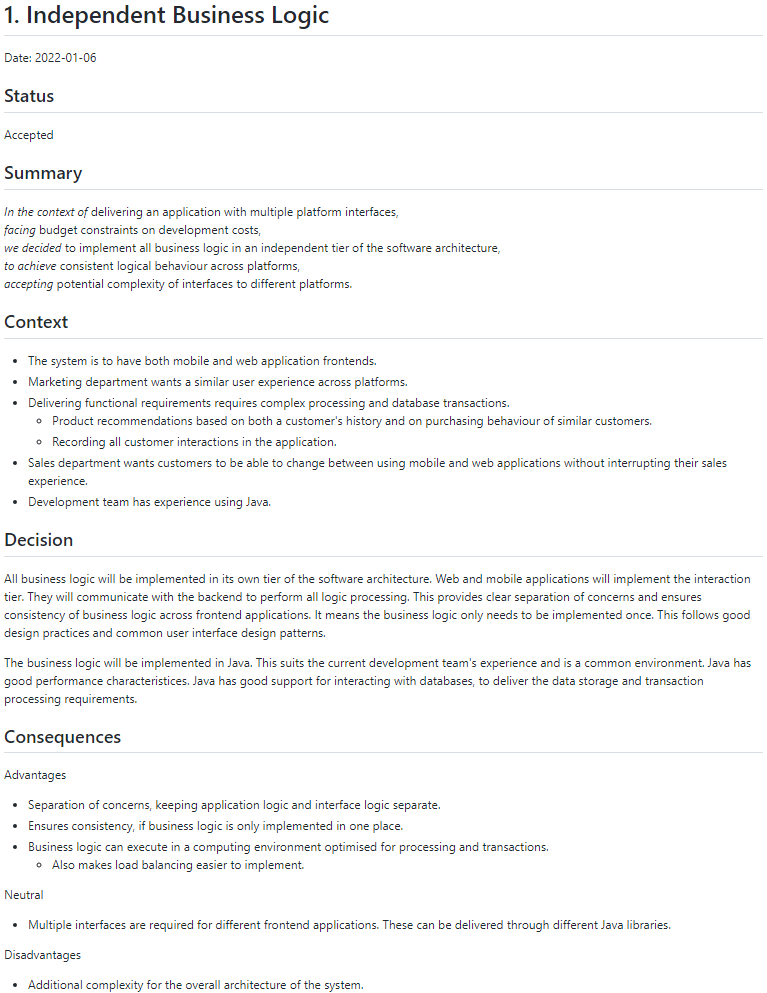
\includegraphics[height=\textheight]{images/adr-example.png}}
\end{figure}

\end{frame}

\note{
    From Sahara example in the views lecture/notes.

    Sahara functional requirement: Ability to change mode of interaction with the system.

    Independent business logic enables this.

    Format of the summary is a why statement --- summarise the context and decision.
}

\point[Reading...]{``Architectural Decision Records'' Notes \cite{adr-notes}}


\references{articles,books,ours}

\end{document}
